\documentclass[twocolumn]{article}
\usepackage[english]{babel}
\usepackage[utf8]{inputenc}
\usepackage{amsmath,amssymb,physics,mathtools,blindtext,graphicx,float}
\usepackage[a4paper,total={7.5in,10in}]{geometry}
\usepackage[labelfont=bf]{caption}

\begin{document}
\begin{large}
\section*{Solving the spherically symmetric Poisson equation using B-splines}
\subsection*{Introduction}
Poisson's equation is given by
\begin{equation}
    \nabla^2\varphi = -\rho/\epsilon_0
\end{equation}
where $\varphi$ is the electric potential, $\rho$ is a charge distribution and $\epsilon_0$ is the permittivity of free space. For a spherically symmetric problem, the equation simplifies to
\begin{equation}
    \frac{\text{d}^2\varphi}{\text{d}r^2}+\frac{2}{r}\frac{\text{d}\varphi}{\text{d}r} = -\rho(r)/\epsilon_0
\end{equation}
and by defining the function $u=r\varphi$, this becomes
\begin{equation}
    \label{12apr1845}
    \frac{\text{d}^2u}{\text{d}r^2} + r\rho(r)/\epsilon_0 = 0.
\end{equation}
A description will now be given on how this equation was solved numerically using B-splines for the following charge distributions:
\begin{itemize}
    \item[1.] A uniformily charged sphere, 
    \begin{equation}
        \rho(r) = 
        \begin{cases}
            3q/(4\pi R^3),\quad r\leq R \\ 
            0,\hspace{1.7cm}\quad r>R
        \end{cases}
    \end{equation}
    where $q$ is the total charge and $R$ is the radius of the sphere.
    \item[2.] A uniformily charged shell,
    \begin{equation}
        \rho(r) = 
        \begin{cases}
            0,\hspace{3.2cm}\quad r<R_1  \\ 
            3q/(4\pi (R_2^3-R_1^3)),\quad R_1\leq r\leq R_2 \\ 
            0,\hspace{3.2cm}\quad r>R_2
        \end{cases}
    \end{equation}
    where $R_1$ and $R_2$ are the inner and outer radii, respectively.
    \item[3.] The electron charge distribution in an hydrogen atom:
    \begin{equation}
        \begin{split}
            &\rho_{1\text{s}}(r) = \frac{q}{\pi a_0^3}e^{-2r/a_0} \\
            &\rho_{2\text{s}}(r) = \frac{q}{32\pi a_0^3}\left(2-\frac{r}{a_0}\right)^2e^{-r/a_0} \\
            &\rho_{3\text{s}}(r) = \frac{q}{3\cdot 81^2\pi a_0^3}\left(27-18\frac{r}{a_0}+\frac{r^2}{a_0^2}\right)^2e^{-2r/3a_0} \\
        \end{split}
    \end{equation}
    where $a_0$ is the Bohr radius.
\end{itemize}


\subsection*{Method}
Since $\varphi(r) = u(r)/r$ and we wish $\varphi(0)$ to be finite, we let $u(0) = 0$. For the first and second charge distributions, we know that $u(r) = q/4\pi\epsilon_0$ outside the enclosing volumes because of Gauss's law. Accordingly, we let $u(R) = q/4\pi\epsilon_0$ for the first distribution and $u(R_2) = q/4\pi\epsilon_0$ for the second distribution. For the third type of distribution, we introduce a cut-off so that $u(\alpha a_0) = q/4\pi\epsilon_0$ where $\alpha$ is some constant which will later be determined such that the error from this approximation becomes negliable. To facilitate the numerical caluclations, the following dimensionless variables were defined:
\begin{equation}
    \begin{split}
        &\xi = r/r_0 \\ 
        &\lambda = u/(q/4\pi\epsilon_0)
    \end{split}
\end{equation}
where $r_0$ is equal to $R$ for the first distribution, $R_2$ for the second distribution and $\alpha a_0$ for the third distribution. Then equation \eqref{12apr1845} can be written as
\begin{equation}
    \lambda''(\xi) + \xi\sigma(\xi) = 0
\end{equation}
where $\sigma = 4\pi r_0^3\rho/q$. The boundary conditions for $\lambda$ are $\lambda(0) = 0$ and $\lambda(1)=1$. Defining a new function, $g(\xi) = \lambda(\xi) - \xi$, we obtain the following boundary value problems:
\begin{equation}
    \label{17apr0918}
    \begin{split}
        &g''(\xi) + \xi\sigma(\xi) = 0 \\ 
        &g(0) = g(1) = 0.
    \end{split}
\end{equation}
These are the equations that were solved for the different charge distributions, $\sigma$.

To do so, a collocation method with B-splines as candidate solutions was used. The numerical solution to $g$ was written as 
\begin{equation}
    \hat{g}(\xi) = \sum_{j=0}^{n-1}c_jB_{j,k}(\xi)
\end{equation}
where $B_{j,k}$ are B-splines of degree $k=3$. Four knot points were placed at $\xi=0$ and another four at $\xi=1$ so that the only non-zero B-spline at $\xi=0$ was $B_{1,k}$ and the only non-zero B-spline at $\xi=1$ was $B_{n,k}$. The boundary conditions were thus satisfied by setting $c_1=c_{n-1}=0$. The other knot points, as well as the collocation points $\xi_k$, were evenly spaced on $(0,1)$. The coefficients were then obtained by solving the linear system of equations:
\begin{equation}
    \begin{split}
        &c_0 = 0, \quad c_{n-1} = 0, \\ 
        &\sum_{j=0}^{n-1}c_jB''_{j,k}(\xi_k) + \xi_k\sigma(\xi_k) = 0,\quad k=1,2\dots,n-2. \\ 
    \end{split}
\end{equation}

\subsection*{Results}
\begin{figure}[b!]
    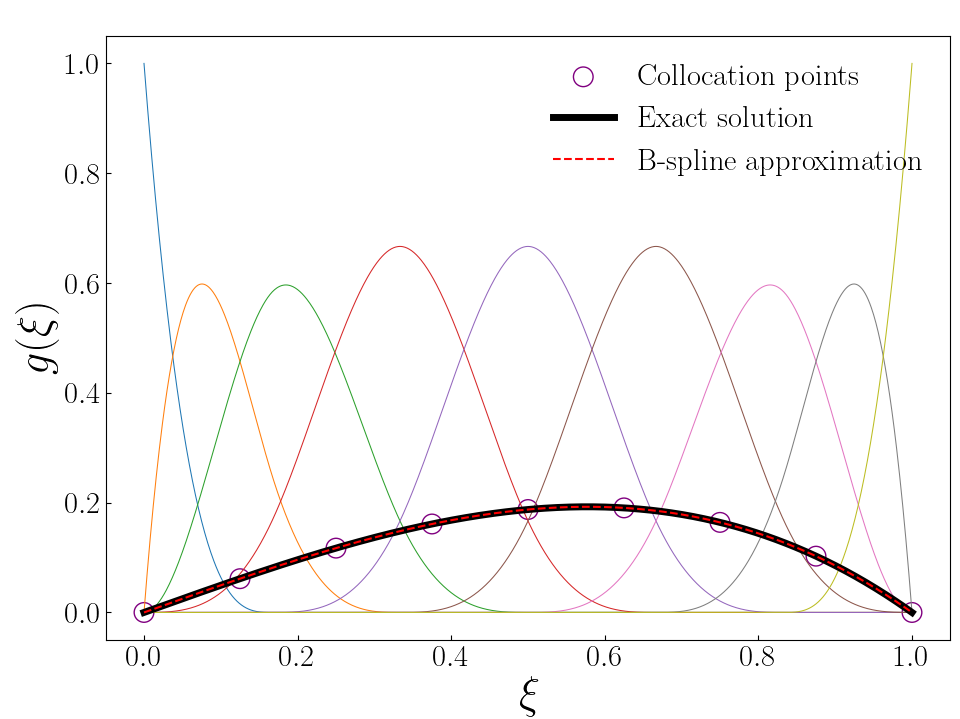
\includegraphics[scale=0.35]{Uniform_g.png}
    \caption{The solution to the boundary value problem given in equation \eqref{17apr0918} for the uniformily charged sphere. Nine B-splines were used (plotted in background) for which the coefficients were $\mathbf{c} = (0,0.028,0.08,0.15,0.19,0.19,0.14,0.056,0)$.}
    \label{17apr0917}
    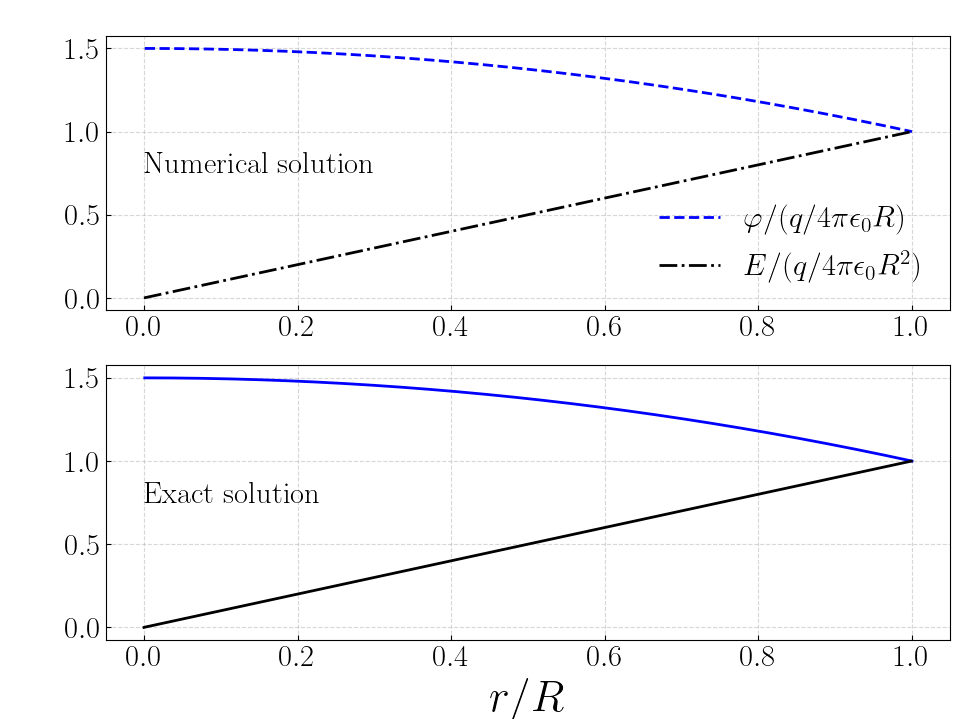
\includegraphics[scale=0.35]{Uniform_EPhi.png}
    \caption{The potential and electric field inside a uniformily charged sphere using B-splines (top) compared to the real solution (bottom).}
    \label{17apr0937}
\end{figure}
The results for the first charge distribution can be seen in figures \ref{17apr0917} and \ref{17apr0937}. In the first figure, the B-spline approximation $\hat{g}$ to the boundary value problem \eqref{17apr0918} is plotted along with the B-splines used and the exact solution $g$ which can be obtained by integrating \eqref{17apr0918} twice. The B-spline approximation was compared to the exact solution and it was found that even for a small number of B-splines ($<10$), the errors in the collocation points were vanishingly small. In the second figure, the electric potential and electric field, (which was obtained by numerically differentiating the potential), are plotted. A similar plot for the second charge distribution is shown in figure \ref{17apr0950} and the same for the hydrogen charge distributions in figures \ref{17apr0959} and \ref{18apr2008}. 
\begin{figure}[b!]
    \includegraphics[scale=0.35]{shell_ephi.png}
    \caption{The electric potential and field inside a shell with inner and outer radii ratio $R_1/R_2=0.5$. The number of B-splines was 84 and the maximum error in the collocation points was $\approx 2\cdot 10^{-5}$.}
    \label{17apr0950}
    \includegraphics[scale=0.35]{hydrogen_ephi.png}
    \caption{The electric potential and field of the electron charge distribution of a hydrogen atom in 1s state. The number of B-splines was 84 and the maximum error in the collocation points was $\approx 3\cdot 10^{-3}$.}
    \label{17apr0959}
    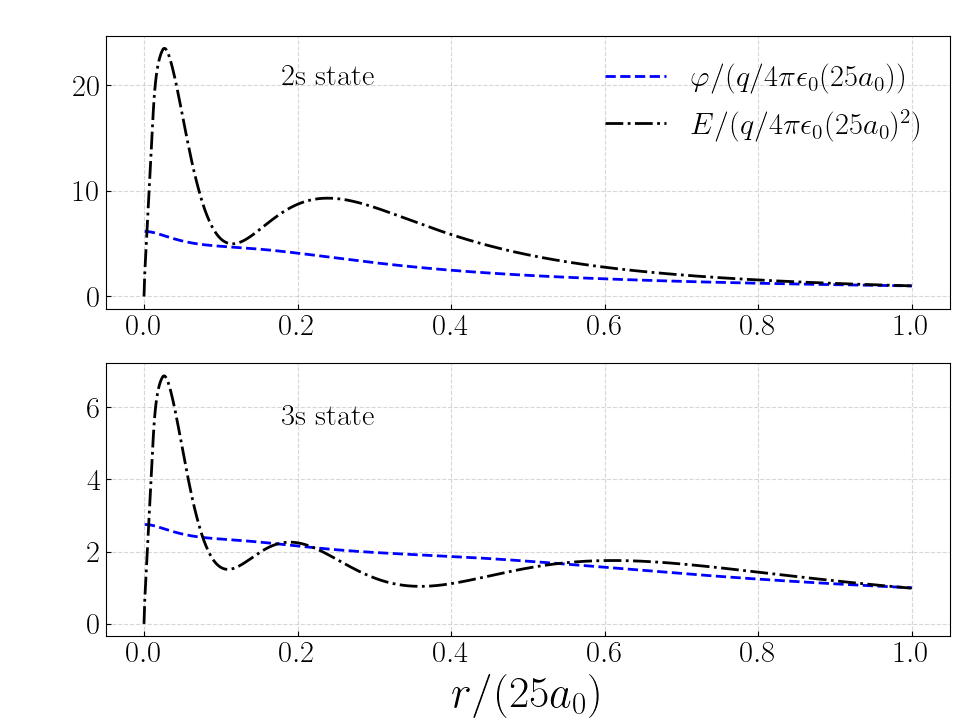
\includegraphics[scale=0.35]{Hydrogen_23.png}
    \caption{The potential and electric field from the electron charge distributions of the 1s and 2s states of hydrogen atom.}
    \label{18apr2008}
\end{figure}

\newpage
The parameter $\alpha$, which determined the length scale for the hydrogen distributions, was chosen such that the electric field satisfied $E\approx q/(4\pi\epsilon_0x^2a_0^2)$ for $x \geq \alpha$. For the 1s, 2s and 3s distributions, it proved sufficient to let $\alpha=25$.

The maximum error of the boundary value problem \eqref{17apr0918} in the collocation points, i.e. \mbox{$\text{max}|g(\xi_k)-\hat{g}(\xi_k)|$}, as a function of the number of splines is plotted in figure \ref{17apr0946}. For the 1s charge distribution, the error decreases with the number of splines and for the charge distribution of the shell, the error seems to oscillate but decrease overall.
\begin{figure}[h!]
    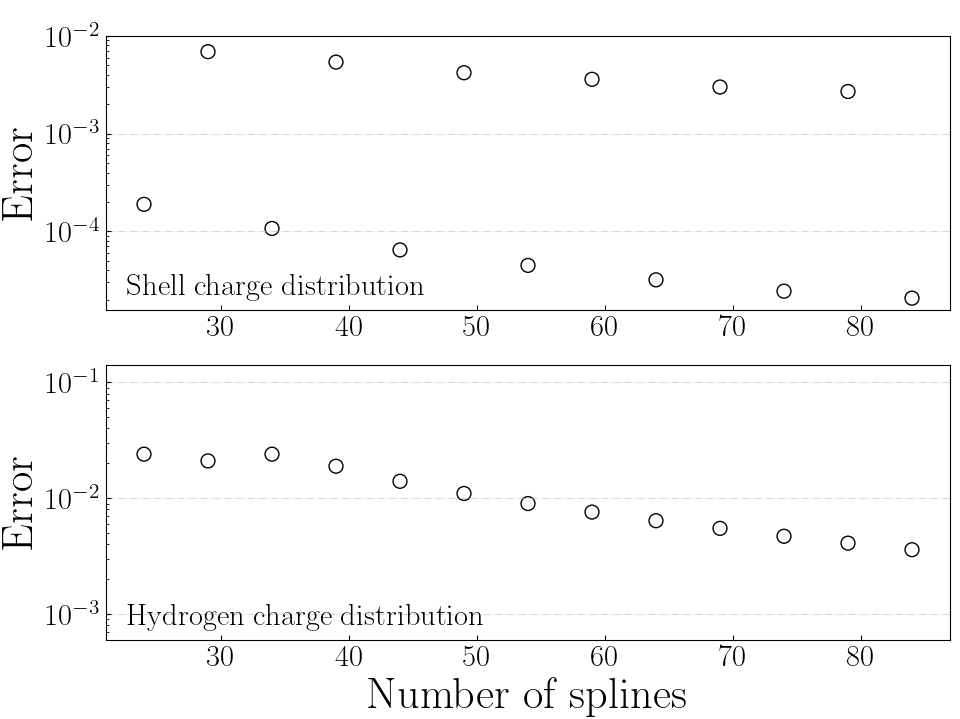
\includegraphics[scale=0.35]{Errors.png}
    \caption{The maximum errors in the collocation points of the shell and hydrogen charge distributions when using the B-spline approximation.}
    \label{17apr0946}
\end{figure}
















\end{large}
\end{document}
